% Créé par Martin Bodin (2011).
% Document sous licence CC BY-NC-SA

% Créé par Martin Bodin (2011).
% Document sous licence CC BY-NC-SA

\documentclass{article}
%\documentclass{scrartcl}

\usepackage{ifxetex}
\ifxetex
\usepackage{xunicode,fontspec,xltxtra}
\else
\usepackage[utf8x]{inputenc}
\usepackage[T1]{fontenc}
\usepackage{amsmath, amsthm}
\usepackage{amsfonts, amssymb}
\fi

\usepackage[francais]{babel}
\usepackage{lmodern}
\usepackage{stmaryrd}
\usepackage{graphicx}
\usepackage[nottoc, notlof, notlot]{tocbibind}
\usepackage[dvipsnames]{pstricks}
\usepackage{pst-circ, pst-plot, pstricks-add}
\usepackage{array}
\usepackage{url}
\usepackage{verse}
\usepackage[colorlinks,linkcolor=black]{hyperref}
\usepackage{ifthen}
\usepackage{longtable, rotating}
%\usepackage{fancyhdr}
\usepackage{fancybox, framed}
\usepackage{textcomp}
\usepackage{marvosym}
%\usepackage{bbding}
%\usepackage{a4wide}
\usepackage{geometry}
%\usepackage{soul}
\usepackage{lettrine}
%\usepackage{yfonts}
\usepackage{oldgerm}
\usepackage{enumerate}
\usepackage{tikz}
\usepackage{dictsym}
\usepackage{pifont}

\ifxetex
\newfontfamily\timesfont[Ligatures=TeX]{Times New Roman}
\setmainfont[Mapping=tex-text, Ligatures={Contextual, Common, Historical, Rare, Discretionary}, Numbers={OldStyle}]{Linux Libertine O}
\fi

%\newcommand{\enluminure}[2]{\lettrine[lines=3]{\small \initfamily #1}{#2}}

\usetikzlibrary{trees}
\usetikzlibrary{arrows,shapes,automata,petri}
\usetikzlibrary{fit}
\usetikzlibrary{calc,decorations.pathmorphing,patterns}


\geometry{
	includeheadfoot,
	margin = 2.54cm,
	top = 1.5cm,
	bottom = 1.5cm
}

\newcommand{\ds}{\displaystyle}

\renewcommand{\ge}{\geqslant}
\renewcommand{\le}{\leqslant}
\renewcommand{\preceq}{\preccurlyeq}
\renewcommand{\succeq}{\succcurlyeq}

\newcommand{\Numero}{\No}
\newcommand{\numero}{\no}

\newcommand{\fixme}{\textbf{FIXME}}

\makeatletter

\newcommand{\defineNewPlayer}[2]{
	\@namedef{couleur#1}{#2}
}

\newcommand{\getPlayerColor}[1]{%
	\@nameuse{couleur#1}%
}

\makeatother

% Des commandes pratiques pour générer le document.
\newcommand{\player}[2]{%
	\ifthenelse{\equal{\forplayer}{y}}{%
		\ifthenelse{\equal{\theplayer}{#1}}%
		{#2}{}%
	}{\begin{barv}[\getPlayerColor{#1}]{2pt}{10pt}#2\end{barv}}%
}
\newcommand{\mj}[1]{%
	\ifthenelse{\equal{\forplayer}{n}}{#1}{}%
}
% Ici suit une commande plus complexe, car plus générale.
\makeatletter

\newcommand{\@beginColor}[3][black]{%
	\ifthenelse{\equal{\forplayer}{n}}{%
		\begin{barv}[#1]{#2}{#3}%
	}{}%
}

\newcommand{\@endColor}{%
	\ifthenelse{\equal{\forplayer}{n}}{%
		\end{barv}%
	}{}%
}


\newcommand{\ignore}[1]{}
\newcommand{\@ident}[3]{%
%	\ifthenelse{\equal{\manyColored}{y}}{#1}{%
%		\marginpar{%
%			#1%
%			\vspace{2cm}%
%			#2%
%		}%
%	}%
	#1%
	\ifthenelse{\equal{\forplayer}{n}}{\@beginColor{0pt}{10pt}}{}%
	#3%
	\ifthenelse{\equal{\forplayer}{n}}{\@endColor}{}%
	#2%
%	\ifthenelse{\equal{\manyColored}{y}}{#2}{%
%		\marginpar{%
%			#1%
%			\vspace{5pt}%
%			#2%
%		}%
%	}%
}

\def\@ouverture#1#2{%
\ifthenelse{\equal{\forplayer}{y}}{}{%
\ifthenelse{\equal{\manyColored}{y}}{\@beginColor[#1]{1pt}{0pt}}{%
\hspace{-1cm}\hspace{-#2mm}\parbox[c][1pt][t]{0pt}{
\begin{tikzpicture}
	\node (a) {};
	\node (b) [right of = a, node distance = 16cm] {};
	\node (c) [below of = a, node distance = 2cm] {};
	\draw [very thick, color = #1] (a.center) -- (b);
	\draw [very thick, color = #1] (a.center) -- (c);
\end{tikzpicture}
}\vspace{-3.2mm}\par%
}%
}%
}
\def\@fermeture#1#2{%
\ifthenelse{\equal{\forplayer}{y}}{}{%
\ifthenelse{\equal{\manyColored}{y}}{\@endColor}{%
\hspace{-1cm}\hspace{-#2mm}\parbox[c][1pt][b]{0pt}{
\begin{tikzpicture}
	\node (a) {};
	\node (b) [right of = a, node distance = 16cm] {};
	\node (c) [above of = a, node distance = 1cm] {};
	\draw [very thick, color = #1] (a.center) -- (b);
	\draw [very thick, color = #1, dashed] (a.center) -- (c);
\end{tikzpicture}
}\vspace{-3.2mm}\par%
}%
}%
}

\def\players@parse#1#2[#3][#4]{%
% #1 :  Suite de \@ouverture
% #2 :  Suite de \@fermeture
% #3 :  Commande à appeler dans le cas d’une réponse négative (≃ réponse précédente).
% #4 :  Argument (sous forme de numéro de joueur) lu actuellement.
	\ifthenelse{\equal{\theplayer}{#4}}{%
		\players@yes{\@ouverture{\getPlayerColor{#4}}{#4}#1}{#2\@fermeture{\getPlayerColor{#4}}{#4}}%
	}{%
		#3{\@ouverture{\getPlayerColor{#4}}{#4}#1}{#2\@fermeture{\getPlayerColor{#4}}{#4}}%
	}%
}

\def\players@no#1#2{%
	\@ifnextchar[{\players@parse{#1}{#2}[\players@no]}{\ignore}%
}

\def\players@yes#1#2{%
	\@ifnextchar[{\players@parse{#1}{#2}[\players@yes]}{\@ident{#1}{#2}}%
}

\def\players{%
	\ifthenelse{\equal{\forplayer}{y}}{%
		\players@no{}{}%
	}{%
		\players@yes{}{}%
	}%
}

% \players{…} est quasi-équivalent à \mj{…}.
% \players[i]{…} est équivalent à \player{i}{…}
% \players[i][j][k]{…} va créer du contenu uniquement pour les joueurs i, j et k (et les MJ bien sûr).

\makeatother
%\fixme :  Ces commandes posent des problèmes pour toutes les sections, footnote, etc. :S

\newcommand{\colorForMJ}[2]{%
	\ifthenelse{\equal{\forplayer}{y}}{#2}{%
		\textcolor{\getPlayerColor{#1}}{#2}%
	}%
}
\newcommand{\synopsisPerso}[3]{%
\paragraph{}{
\textbf{\fcolorbox{\getPlayerColor{#1}}{white}{#2}}\hspace{10pt}%
{#3}}%
}

\newenvironment{changemargin}[2]{\begin{list}{}{%
\setlength{\topsep}{0pt}%
\setlength{\leftmargin}{0pt}%
\setlength{\rightmargin}{0pt}%
\setlength{\listparindent}{\parindent}%
\setlength{\itemindent}{\parindent}%
\setlength{\parsep}{0pt plus 1pt}%
\addtolength{\leftmargin}{#1}%
\addtolength{\rightmargin}{#2}%
}\item }{\end{list}}
\reversemarginpar
%\pagestyle{fancy}
%\fancyhf{}
%\renewcommand{\headrulewidth}{0pt}
%\lhead{}
%\lfoot{}

\makeatletter
\newenvironment{barv}[3][black]{%
% #2 largeur du trait
% #3 distance entre le trait et le texte
	\def\FrameCommand{{\color{#1}\vrule width #2}
	\hspace{#3}}%
	\MakeFramed {\advance \hsize -\width \FrameRestore }%
}{%
    \endMakeFramed%
}
\makeatother


\definecolor{LightButter}{rgb}{0.98,0.91,0.31}
\definecolor{LightOrange}{rgb}{0.98,0.68,0.24}
\definecolor{LightChocolate}{rgb}{0.91,0.72,0.43}
\definecolor{LightChameleon}{rgb}{0.54,0.88,0.20}
\definecolor{LightSkyBlue}{rgb}{0.45,0.62,0.81}
\definecolor{LightPlum}{rgb}{0.68,0.50,0.66}
\definecolor{LightScarletRed}{rgb}{0.93,0.16,0.16}
\definecolor{Butter}{rgb}{0.93,0.86,0.25}
\definecolor{Orange}{rgb}{0.96,0.47,0.00}
\definecolor{Chocolate}{rgb}{0.75,0.49,0.07}
\definecolor{Chameleon}{rgb}{0.45,0.82,0.09}
\definecolor{SkyBlue}{rgb}{0.20,0.39,0.64}
\definecolor{Plum}{rgb}{0.46,0.31,0.48}
\definecolor{ScarletRed}{rgb}{0.80,0.00,0.00}
\definecolor{DarkButter}{rgb}{0.77,0.62,0.00}
\definecolor{DarkOrange}{rgb}{0.80,0.36,0.00}
\definecolor{DarkChocolate}{rgb}{0.56,0.35,0.01}
\definecolor{DarkChameleon}{rgb}{0.30,0.60,0.02}
\definecolor{DarkSkyBlue}{rgb}{0.12,0.29,0.53}
\definecolor{DarkPlum}{rgb}{0.36,0.21,0.40}
\definecolor{DarkScarletRed}{rgb}{0.64,0.00,0.00}
\definecolor{Aluminium1}{rgb}{0.93,0.93,0.92}
\definecolor{Aluminium2}{rgb}{0.82,0.84,0.81}
\definecolor{Aluminium3}{rgb}{0.73,0.74,0.71}
\definecolor{Aluminium4}{rgb}{0.53,0.54,0.52}
\definecolor{Aluminium5}{rgb}{0.33,0.34,0.32}
\definecolor{Aluminium6}{rgb}{0.18,0.20,0.21}

\pgfdeclarelayer{foreground} 
\pgfdeclarelayer{background} 
\pgfsetlayers{background,main,foreground} 



\newcommand{\forplayer}{y} % or y
\newcommand{\theplayer}{12} % if \equal{\forplayer}{y}, then it represents the number of this player.
\newcommand{\manyColored}{n}

\defineNewPlayer{1}{Red} % Le représentant de la couronne.  Lord Henry Hasting.
\defineNewPlayer{2}{Blue} % Un espion français.  Robert Hatley.
\defineNewPlayer{3}{OliveGreen} % Un industriel curieux.  Thomas Bellford. (Un nom à trouver, mais avec une attache historique faible)
\defineNewPlayer{4}{Cyan} % Le médecin.  (Un nom à trouver, si possible avec une attache historique → Mickaela Owen.  À l’époque, il vient juste de se faire accuser de plagiat.  En recherchant un remède contre la mort, il est sûr de ne pas avoir d’ennui.  Il fait des expériences sur des spongiaires, mais il aimerait se préoccuper d’animaux plus… volumineux.)
\defineNewPlayer{5}{Brown} % John Stringfellow, ingénieur.
\defineNewPlayer{6}{Yellow} % Elisabeth Henson, l’investisseuse qui a réussi à faire croire à tout le monde que c’est lui l’auteur de la machine.
\defineNewPlayer{7}{Plum} % L’organisateur.  Andrew McMahon.  (idem, une attache historique faible.)
%\defineNewPlayer{8}{Gray} % Le responsable de la sécurité.  Frederic Murray. (un nom sans attache).
\defineNewPlayer{9}{BlueViolet} % Charles Wheatstone, qui croit à l’électricité.
\defineNewPlayer{10}{Rhodamine} % La femme de l’organisateur.   Brenda McMahon.  (nom à trouver avec l’organisateur).
%\defineNewPlayer{11}{Violet} % Le savant fou.  Douglas Winterley.  (personnage à améliorer).
\defineNewPlayer{12}{DarkSkyBlue} % La correspondante française de l’organisateur.  Élaine LeGris.  (à trouver).
%\defineNewPlayer{13}{LightBlue} % Un prêtre.  George Compton. (sans attache, quoi que ?)

\newcommand{\pageForPlayer}[5][n]{%
\player{#2}{
	\mj{\newpage}%
	\ifthenelse{\equal{#1}{y}}{\section{Ton perſonnage~: #3}}{\section{Ton personnage~: #3}}
	\begin{description}
			#4
	\end{description}
\par
	\ifthenelse{\equal{#1}{y}}{\paragraph{Deſcription du perſonnage par lui-même.}}{\paragraph{Description du personnage par lui-même.}}
	{#5}
}}

\title{Un Monoplane automatisé}
\author{Martin \textsc{Bodin}}
\date{}

\begin{document}

\mj{\maketitle}

%\tableofcontents

%\newpage

\mj{
\section{À propos de l’univers}

\subsection{Présentation rapide}

Tout se situe dans une uchronie où Charles \textsc{Babbage} aurait réussi à construire un ordinateur en 1835.
Ce dernier fonctionnerait à l’aide de vapeur sous pression et d’engrenages au lieu d’électronique.
À partir de ce nouvel apport à la science et à l’ingénierie les progrès en technologie à engrenage et vapeur ont été considérables, notamment du point de vue de la miniaturisation, à tel point que les scientifiques commencent à apercevoir de légères anomalies dues à des phénomènes quantiques dans leurs ordinateurs (mais ils n’arrivent pas encore à les expliquer).
La technologie de cet univers équivaut à peu près à celle que l’on avait dans le début des années 1960 (ils ont donc plus d’un siècle d’avance sur nous).
La grande différence étant que l’électricité en est réduit au rôle de transfert d’informations sur de longues distances plutôt qu’effectuer les calculs, un peu comme la lumière des fibres optiques dans notre monde.

Cette murder se situera en \textsc{Angleterre}, à \textsc{Wellingborough} (situé à une centaine de kilomètres du Nord de \textsc{Londres}), dans les jardins du Sir~\textsc{McMahon}, le 3 Février 1848.
L’\textsc{Angleterre} est maintenant le pays le plus en avance technologique de toute l’Europe (et donc du monde), la Société Royale d’Astronomie possédant les droits d’utilisation sur l’ordinateur de \textsc{Babbage} et continuant d’investir des sommes colossales afin de rester à la pointe de la technologie.

\subsection{Histoire}

Voici un résumé des principaux événements de l’époque\footnote{
La plupart des événements cités ici ce sont réellement passés, la réalité allant dans le sens d’une avancée technologique britannique de toute façon, il est fort probable que l’invention de l’ordinateur dès 1835 n’ai pas radicalement changé les conflits diplomatiques et économiques.
On peut considérer que tous les événements ne concernant pas les avancées technologiques datant d’après 1821 sont ici historiques (éventuellement simplifiés pour la cause).
}.
Beaucoup ne sont pas en rapport directes avec le scénario, mais comme le scénario va un peu parler de relations internationales, il est bon de connaître le contexte.
Notez bien l’âge de votre personnage (en 1848)~: certains événements l’ont probablement plus marqué que d’autres.

\newcommand{\decouvertes}{\tikz[baseline]\node[fill=LightChameleon!70, rectangle, rounded corners = 1mm]{\Biohazard};}%\dschemical}
\newcommand{\industries}{\tikz[baseline]\node[fill=LightPlum!70, rectangle, rounded corners = 1mm]{\Industry};}%\dsrailways}
\newcommand{\loies}{\tikz[baseline]\node[fill=LightSkyBlue!70, rectangle, rounded corners = 1mm]{\WritingHand};}%\dsjuridical}
\newcommand{\loiesloins}{\tikz[baseline]\node[fill=LightChocolate!70, rectangle, rounded corners = 1mm]{\Mundus};}
\newcommand{\conflits}{\tikz[baseline]\node[fill=LightScarletRed!70, rectangle, rounded corners = 1mm]{\Cross};}%\dsmilitary}
\newcommand{\conflitsloins}{\tikz[baseline]\node[fill=LightOrange!70, rectangle, rounded corners = 1mm]{$\lightning$};}

Pour simplifier la (re-)lecture de cette chronologie, j’ai ajouté les symboles suivants pour bien repérer quel type d’événement est décrit :  \decouvertes{} pour les découvertes scientifiques, \industries{} pour leurs applications industrielles, \loies{} pour les changements politiques des pays proches, \loiesloins{} pour les pays lointains, \conflits{} pour les conflits proches et \conflitsloins{} pour les conflits lointains (donc mineurs pour le scénario).

%\begin{changemargin}{0cm}{0cm}
\xdef\executeStuff{n}
\newcommand{\waitForExecution}[2]{\ifthenelse{\equal{\executeStuff}{y}}{#1{#2}}{\noexpand\waitForExecution{#1}{#2}}}
\newcommand{\myspace}{\hspace{5mm}}
\xdef\toBeExecutedAtChronoline{0/0}
\newcommand{\chronoline}[4]{%
	\def\minDate{#2}%
	\def\maxDate{#4}%
	\def\minDateName{#1}%
	\def\maxDateName{#3}%
	\begin{tikzpicture}[remember picture, overlay]
		\begin{pgfonlayer}{background}
		\shade [top color = LightPlum, bottom color = Plum]
		(\minDateName) ++ (-1.2, 0.8) --
		++(.4, 0) --
		(-1.45, -.8) ++ (\maxDateName) --
		cycle ;
		\end{pgfonlayer}
		\foreach \date in {\minDate,...,\maxDate}{
			\pgfmathparse{(\date - \minDate) / (\maxDate - \minDate)} \let\myPos\pgfmathresult
			\draw[opacity = 0] (\minDateName) ++ (-1, .5) -- (-1.45, -.5) ++ (\maxDateName) node [pos = \myPos, opacity = 1, left = 3mm] (date\date) {\date} ;
		}
		\begin{pgfonlayer}{foreground}
		%\def\executeStuff{y}
		%\toBeExecutedAtChronoline
		\foreach \chrono/\point in \toBeExecutedAtChronoline{
			\ifthenelse{\equal{\chrono}{0}}{}{
				\correspondance{\chrono}{\point}
			}
		}
		\end{pgfonlayer}
	\end{tikzpicture}%
	%\xdef\executeStuff{n}
	\xdef\toBeExecutedAtChronoline{0/0}%
}
\newcommand{\correspondance}[2]{
	%\begin{tikzpicture}[remember picture, overlay]
		%\pgfmathparse{(#1 - \minDate) / (\maxDate - \minDate)} \let\myPos\pgfmathresult
		%\draw[opacity = 0] (#1) ++ (-1, .5) -- (-1, -.5) ++ (#3) node [pos = \myPos, opacity = 1, right = 3mm] -- (#2) ;
		%\draw[->, thick, Chameleon] (date#1) -- (#2) ;
	%\end{tikzpicture}
	\draw[->, thick, DarkPlum, opacity = 1] (#1.east) + (0.3,0) .. controls +(.6, 0) and +(-1, 0) .. (#2.west) ;
}
\xdef\currentNumberOfNode{O}
\newcommand{\evenement}[5][]{
	\ifthenelse{\equal{#1}{}}{}{%
		\makebox[0pt]{\tikz[remember picture] \node (#1) {} ;}
	}%
	\tikz[remember picture] \node (node\currentNumberOfNode) {} ;
	%\ifthenelse{\equal{\@nameuse{date#2}}{}}{\@namedef{date#2}{node\currentNumberOfNode}}{%
	%	\makeatletter%
		%\fixme
		%\def\oldNodes{\@nameuse{date#2}}%
		%\@namedef{date#2}{\oldNodes, node\currentNumberOfNode}%
	%	\makeatother%
	%}%
	%\xdef\toBeExecutedAtChronoline{\toBeExecutedAtChronoline\waitForExecution{\noexpand\correspondance}{{#2}{node\currentNumberOfNode}}}%
	\xdef\toBeExecutedAtChronoline{date#2/node\currentNumberOfNode,\toBeExecutedAtChronoline}%
	%\show\toBeExecutedAtChronoline%
	%\pgfmathparse{\currentNumberOfNode + 1}\xdef\currentNumberOfNode{\pgfmathresult}%
	\xdef\currentNumberOfNode{S\currentNumberOfNode}%
	%\show\currentNumberOfNode%
	#5%
	#3 &
	#2 &
	$
	\left\{
		\myspace{}
		\parbox{12.8cm}{ % 9cm pour le mode non a4wide.
			\vspace{1mm}#4\vspace{1mm}
		}
	\right.
	$ \\[3mm]
}

%\sethlcolor{LightButter}
%\newcommand{\important}[1]{\hl{#1}}

\newcommand{\important}[1]{\tikz[baseline = -0.8ex]
	\node [rectangle, fill = LightButter, rounded corners = 1mm] {#1};}

%\newcommand{\important}[1]{
%	\begin{tikzpicture}[baseline=-0.1cm]
%		 \node[rectangle,fill,color=LightButter,
%		 rounded corners=1mm] {{#1}};
%	 \end{tikzpicture}%
%}

\setlongtables
\begin{longtable}{llm{13.5cm}} % 10cm pour le mode non a4wide.
& Année & \myspace{} Événement \\
\endfirsthead
& Année & \myspace{} Événement \\
\endhead
\endfoot
\evenement[debut1]{1775}{\industries}{Première adaptation industrielle de \important{la machine à vapeur} de \textsc{James~Watt}.}{}
\evenement{1783}{\industries}{\important{Le premier bateau à vapeur} est inauguré.  À cause de leur faible autonomie, ces bateaux ne circulent que sur les rivières.}{}
\evenement{1789}{\loies}{\important{Abolition des privilèges} des nobles en \textsc{France}}{}
\evenement{1791}{\loies}{Première \important{législation sur les brevets} en \textsc{France} (le Royaume-Uni ayant près d’un siècle d’avance sur la \textsc{France} sur ce point).}{}
\evenement[fin1]{1792}{\decouvertes}{\textsc{George~Cayley} énonce les principes théoriques pour qu’un véhicule volant soit construit.}{\chronoline{debut1}{1775}{fin1}{1792}}
\evenement[debut2]{1793}{\conflits}{Régime de \important{la Terreur} en \textsc{France}.}{}
\evenement{1796}{\decouvertes}{Découverte du \important{procédé de vaccination} antivariolique par \textsc{Edward~Jenner}.}{}
\evenement{1799}{\loies}{\important{\textsc{Napoléon} prend le pouvoir} en \textsc{France} et établit son Consulat.}{}
\evenement{1800}{\loies}{Le brevet de \textsc{Watt} sur sa machine à vapeur tombe dans le domaine public. Près de \important{500 machines sont en services} en Grande-Bretagne.}{}
\evenement{1804}{\loies}{\textsc{Napoléon I$^\textrm{er}$} est \important{déclaré Empereur} de \textsc{France}.}{}
\evenement{1804}{\industries}{Le \important{premier train à vapeur}, construit par \textsc{Richard~Trevithick}, circule pour la première fois, au Pays de Galles.}{}
\evenement{1806}{\conflits}{\textsc{Napoléon I$^\textrm{er}$}, qui cherche à asphyxier économiquement le Royaume-Uni en annexant l’Europe continentale, arrive à l’apogée de son royaume.  Une bonne partie de l’Europe est sous domination du \important{grand Empire}.}{}
\evenement{1806}{\decouvertes}{Découverte de la morphine.}{}
\evenement{1806}{\conflits}{\textsc{Napoléon I$^\textrm{er}$} instaure un \important{blocus continental} en bloquant les ports importants ayant un contact avec la Grande-Bretagne.}{}
\evenement{1808}{\decouvertes}{Humphry \textrm{Davy} isole le sodium, le potassium, le baryum, le strontium et le calcium grâce à \important{l’électrolyse}.  Il fera aussi de très nombreuses découvertes en médecines et en physique des gaz dans les années qui suivent.}{}
\evenement{1812}{\conflitsloins}{\important{Guerre d’indépendance des États-Unis} contre l’Empire britannique.}{}
\evenement{1815}{\conflits}{\important{\textsc{Napoléon I$^\textrm{er}$} est vaincu à \textsc{Waterloo}} et les frontières françaises redeviennent plus ou moins dans la normale comme le stipule traité de \textsc{Vienne}.  Le traité met aussi en avant la neutralité de la Suisse.  \textsc{Louis XVIII} devient roi de \textsc{France}. }{}
\evenement{1820}{\loies}{\important{Le roi \textsc{George IV}} succède à \textsc{George III} au Royaume-Uni.}{}
\evenement{1821}{\decouvertes}{\textsc{Charles~Babbage} présente un modèle de sa machine à différences à la Société Royale d’Astronomie.  Il obtient une bourse conséquente pour la réalisation de son projet.}{}
\evenement{1823}{\decouvertes}{La \important{première machine à différence} est construite.}{}
\evenement{1824}{\loiesloins}{Le traité de 1814 entre l’Angleterre et la Hollande — qui définissait des limites et accords sur le développement colonial des deux nations — apportant de nombreux litiges, un nouveau est rédigé.}{}
\evenement{1824}{\loies}{\important{\textsc{Charles X}} succède à \textsc{Louis XVIII} en \textsc{France}, qui tente de rétablir l’ancien Régime.}{}
\evenement{1825}{\loies}{\important{Le droit de grève} des ouvriers est acquis en Angleterre.}{}
\evenement{1826}{\decouvertes}{\textsc{Charles~Babbage} conçoit un modèle optimisé de sa machine à différence ne demandant que trois fois moins de pièces.}{}
\evenement[fin2]{1827}{\loiesloins}{\important{Le traité de Londres} entre le Royaume-Uni, la \textsc{France} et la Russie est signé.  Il vise à réduire l’influence turque en Europe en libérant la Grèce de son emprise contestée.}{\chronoline{debut2}{1793}{fin2}{1827}}
\evenement[debut3]{1828}{\decouvertes}{À l’aide des travaux d’\textsc{Ada~Lovelace} et de \textsc{Charles~Babbage}, ainsi que des financements du Royaume-Uni par la \textsc{Royal Society}, \important{les premiers programmes informatiques} commencent à être écrits.}{}
\evenement{1830}{\conflitsloins}{\important{Des tensions} entre la Pologne et la Russie, ainsi qu’entre la Belgique et les Pays-Bas éclatent.  Le soutien de la \textsc{France} est beaucoup demandé, mais les autres Puissances préfèrent que la \textsc{France} ne s’occupe pas trop des conflits militaires des autres nations.}{}
\evenement{1830}{\loies}{\important{Le roi \textsc{Guillaume IV}} succède à \textsc{George IV} au Royaume-Uni.}{}
\evenement{1830}{\loiesloins}{Naissance officielle de la Grèce.}{}
\evenement{1830}{\loies}{\important{Révolution en \textsc{France}}~:  \textsc{Louis-Philippe} devient roi des Français.  Le drapeau français devient tricolore.}{}
\evenement{1830}{\industries}{Le Royaume-Uni possède maintenant plus de \important{15~000 machines à vapeur}, contre seulement 3~000 en \textsc{France} et 1~000 en Prusse.}{}
\evenement{1830}{\decouvertes}{À la demande de \textsc{Babbage}, \textsc{Joseph-Marie~Jacquard} est subventionné par la \textsc{Royal Society} pour aider \textsc{Babbage} à concevoir \important{un nouveau modèle de carte perforées} qui permettrait une programmation plus simple de sa machine.}{}
\evenement{1831}{\loies}{\important{Le traité des XVIII articles}, qui reconnaît officiellement la séparation de la Belgique et des Pays-Bas et fait de la Belgique un pays neutre, est signé par les Puissances.}{}
\evenement{1831}{\loiesloins}{La Pologne est déclarée indépendante.  Le Royaume-Uni craint une extension de l’influence française qui pourrait entraîner d’autres \important{révolutions anti-monarchiques}.}{}
\evenement{1831}{\decouvertes}{\textsc{Michael~Faraday} découvre le phénomène d’\important{induction électromagnétique}.}{}
\evenement{1832}{\loies}{La \textsc{France} affirme qu’elle est désormais en mesure de mener une politique autonome.}{}
\evenement{1832}{\loies}{La \textit{Reform Bill} au Royaume-Uni, réforme qui augmente le nombre de votant en diminuant la franchise électorale, mais sans la supprimer.  Les classes populaires voient \important{la faiblesse des réformes} comme une trahison de leurs représentants bourgeois.}{}
\evenement{1833}{\industries}{Les industriels commencent à s’intéresser aux travaux de \textsc{Babbage} et \textsc{Lovelace} et de nombreuses compagnies se mettent à utiliser moyennement gros financements ces machines pour concevoir \important{des modèles d’ingénierie}.}{}
\evenement{1833}{\decouvertes}{\textsc{Faraday} énonce les bases de l’\important{électrochimie}.}{}
\evenement{1834}{\loies}{\important{Traité de la Quadruple Alliance}, une alliance militaire tant défensive qu’offensive, est signé entre le Royaume-Uni, la \textsc{France}, l’Espagne et le Portugal.}{}
\evenement{1835}{\industries}{\textsc{Babbage} et \textsc{Jacquard} conçoivent un véritable (facilement reprogrammable) \important{calculateur à vapeur}, utilisable (et conçu) pour les calculs de l’industrie et les calculs militaires.  \textsc{Lovelace} a apporté un travail énorme pour la programmation de nombreuses cartes perforées.}{}
\evenement{1836}{\industries}{\textsc{Charles~Wheatstone} met en place \important{la première liaison télégraphique} filaire, au nord de Londres.}{}
\evenement[fin3]{1837}{\loies}{\important{La reine \textsc{Victoria}} succède à \textsc{Guillaume IV} au Royaume-Uni.}{\chronoline{debut3}{1828}{fin3}{1837}}
\evenement[debut4]{1838}{\loies}{Un traité commercial entre le Royaume-Uni, la \textsc{France} et l’empire ottoman aboli tout privilège commercial, ceci ouvre au Royaume-Uni toutes les portes d’une \important{grande influence commerciale}.}{}
\evenement{1838}{\loies}{L’Union nationale du travail, un syndicat regroupant les ouvriers dont le but est de supprimer la classe patronale vient de naître.  Les industriels brisent le mouvement dans la foulée.}{}
\evenement{1840}{\decouvertes}{\textsc{Elisabeth~Henson} à l’aide de \textsc{John~Stringfellow}, s’appuyant sur les travaux de \textsc{Cayley}, conçoit les plans complets d’\textsc{Ariel}, \important{une machine volante à vapeur} et essait de trouver des fonds pour le construire.}{}
\evenement{1840}{\loies}{Le Royaume-Uni voulant supprimer la traite des noirs, il créé la \important{Convention de Londres} qui abolit l’esclavage.  La \textsc{France} ayant beaucoup d’actions dans les navires négriers refuse de ratifier cet accord.}{}
\evenement{1840}{\conflitsloins}{Les vainqueurs de 1815 (le Royaume-Uni, la Russie, l’Autriche et la Prusse) signent un traité pour redonner l’Égypte, où la \textsc{France} avait une influence très importante, à son ancien souverain.}{}
\evenement{1842}{\decouvertes}{\textsc{Faraday} met au point un système à base de réactions chimiques relativement complexes utilisant l’«~instabilité de Faraday~» permettant de convertir des signaux de pression en des signaux électriques~:  il est maintenant possible (du moins en théorie) de créer des \important{ordinateurs qui s’échangent des informations} sur de longues distances (à la manière d’Internet).}{}
\evenement{1844}{\conflitsloins}{Un \important{conflit anglo-français} à Tahiti, alors colonie française, éclate.}{}
\evenement{1845}{\decouvertes}{\textsc{Faraday} améliore son système chimique~:  il est maintenant possible de construire \important{une mémoire} à grande capacité et rapidité de lecture pour la machine.}{}
\evenement[fin4]{1846}{\industries}{\textsc{Babbage} et \textsc{Faraday} conçoivent \important{le premier exemplaire de l’«~ordinatrice~»}.  Cette machine relativement portable (elle mesure environ deux mètres de long pour un mètre de haut) est capable de faire des calculs à grande vitesse pour tous les types d’applications.  Sa principale caractéristique est qu’elle est constructible à la chaîne.  Les industriels s’empressent de lancer sa production à grande échelle.}{\chronoline{debut4}{1838}{fin4}{1846}}
\end{longtable}
%\end{changemargin}

%\fixme:	\player{12}{1846 & À la suite de mauvaises récoltes, la France connaît une crise économique profonde. \\

Voici maintenant une carte du monde de l’époque.
Sur cette carte, l’Empire Britannique est représenté en rouge~:
\begin{center}
	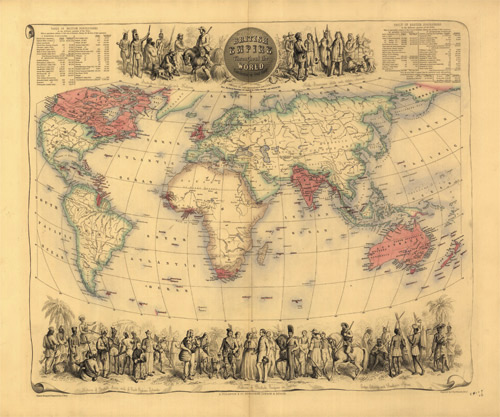
\includegraphics[width = 10cm]{world.jpg}
\end{center}

\subsection{Synopsis}

Sir~\textsc{Andrew~McMahon} nous convie tous à une des ses expositions des nouvelles technologies, comme c’est maintenant beaucoup à la mode.
Il a pour cela réorganisé tous ses jardins du compté de \textsc{Wellingborough}~:  rien ne pourra déranger les invités pendant qu’ils admirent ces nouvelles technologies.
On peut d’ors et déjà apercevoir les différentes machines de vapeur s’aligner par ici.
La forge est située suffisamment loin pour qu’elle ne nous dérange pas et de nombreux tuyaux de cuivre transmettent la pression jusqu’aux machines.

La vedette de cette exposition est un prototype de machine volante à vapeur, présenté par Sir~\textsc{Elisabeth~Henson}.
Elle permettrait à l’aide d’un unique homme de transporter de nombreuses charges sur de très longues distances.
Imaginez ce que cela pourra apporter à la déjà très puissante économie d’\textsc{Angleterre}~!
Son coût élevé devrait rapidement être rentabilisé par de telles fonctionnalités.
Mais bien entendu, ceci n’est qu’un prototype…


\subsection{Les différents personnages}

Voici les différents personnages présents à l’exposition~:
\begin{description}
\item[Lord~\textsc{Henry~Hasting}, 73~ans] Représentant direct de la Couronne, il nous fait l’honneur d’être venu découvrir lui aussi ces nouvelles inventions.
\item[\textsc{Robert~Hatley}, 26~ans] Noble du \textsc{Wiltshire}, un des visiteurs fortunés intéressés par ces découvertes.
\item[\textsc{Thomas~Bellford}, 52~ans] Un industriel du \textsc{Suffolk}, probablement intéressé par de nouvelles sources d’investissement…
\item[\textsc{Dr~Mickaela~Owen}, 43~ans] Médecin tout droit sorti de l’\textsc{Université de Londres} qui profite de cet événement pour venir exposer ses nouvelles théories.
\item[\textsc{John~Stringfellow}, 50~ans] Ingénieur, responsable de la machine volante.
\item[\textsc{Elisabeth~Henson}, 35~ans] Investisseuse, inventrice de la machine volante.
\item[\textsc{Andrew~McMahon}, 63~ans] Grand organisateur de cette exposition.
%\item[\textsc{Frederic~Murray}, 32~ans] Responsable de la sécurité lors de cette exposition.
\item[\textsc{Charles~Wheatstone}, 45~ans] Un physicien de \textsc{Gloucester}.
\item[\textsc{Brenda~McMahon}, 56~ans] Épouse d’\textsc{Andrew~McMahon}.
%\item[\textsc{Douglas~Winterley}] 
\item[\textsc{Élaine~LeGris}, 33~ans] Un actionnaire français.
%\item[\textsc{George~Compton}] Le prêtre de \textsc{Wellingborough} sera lui aussi présent à cet événement.
\end{description}
}

\mj{
\vfill

\foreach\i in {,}{\vfill

\begin{center}
\begin{tikzpicture}
	\node [rectangle, draw = DarkButter, very thick, top color = LightButter, bottom color = LightButter!30, decorate, decoration = {random steps, segment length = 4pt, amplitude = 2pt}] {
		\parbox{14cm}{
			\vspace{5mm}\centering\parbox{13cm}{

\begin{center}
\tikz
\node[fill = Butter, draw = DarkButter, rounded corners = 5mm]
{{\Huge☙}\parbox{8cm}{
	\centering
	\lettrine{\textgoth{E}}{xposition} organisée par \textsc{Andrew~McMahon}\\
	3~Février~1848 \\
	Jardins de \textsc{Wellingborough}
}{\Huge❧}};
\end{center}
 
\lettrine{\textgoth{P}}{rogramme}
\begin{center}
	\begin{tabular}{lm{10cm}}
		13h–13h30 & \textgoth{A}ccueil des participants \\
		13h30 & \textgoth{D}iſcours d’\textsc{Andrew~McMahon} \\
		14h–15h & \textgoth{O}uverture de l’exposition par les exposés de \textsc{Charles~Wheatſtone} et ceux du Docteur~\textsc{Mickaela~Owen} \\
		15h & \textgoth{H}iſtorique de l’innovation ſcientifique, par \textsc{Elisabeth~Henson} \\
		15h30 & \textgoth{P}résentation de la ſituation politique de l’Europe par \textsc{Élaine~LeGris} \\
		16h & \textgoth{P}remiers appels à inveſtiſſements \\
		16h30–17h & \textgoth{T}hé \\
		17h & \textgoth{P}remiers teſts du monoplane par \textsc{Elisabeth~Henson} et ſon ingénieur, \textsc{John~Stringfellow} \\
		18h & \textgoth{S}econds appels à inveſtiſſements \\
		19h & \textgoth{D}iſcours de cloture par \textsc{Andrew~McMahon} \\
	\end{tabular}
\end{center}

}\vspace{5mm}
}} ;
\end{tikzpicture}
\end{center}}
}

\newpage
\pageForPlayer[y]{1}{Lord~Henry~Haſting}{
\item[Âge] 73~ans (né le 15~Juillet~1774).
\item[Détails physiques] Habillé très richement.
\item[Poſſeſſions] Beaucoup d’argent, ainſi que de nombreuses terres tout le long de l’\textsc{Angleterre}.
}{
Ah~!
Quel ennui.
Je rêve encore de \textsc{Londres} et de ſes palais…
Cela ne fait pourtant pas longtemps que je ſuis parti~:  avec le train, maintenant on peut traverſer l’\textsc{Angleterre} toute entière en moins d’un jour~!
Mais quelle paperaſſe il faut pour obtenir cette ſimple place dans le train…  et j’étais loin d’être ſeul dans ce bruyant moyen de tranſport~!

Je regrette tellement mes jeunes années~!
À ce moment là, les choses étaient très ſimples~:  il y avait le Roi~\textsc{George~III} et le reste du monde, qui obéiſſait au Roi.
J’ai fait mes débuts dans cette cour où tout était très carré et bien étudié.
À cette époque, ſi j’avais besoin d’aller en province, ça aurait été beaucoup plus ſimple~:  je demandais une voiture à chevaux qui m’était mise à diſposition immédiatement.
Certes, le voyage était plus long, mais beaucoup plus confortable.

Maintenant, depuis que les induſtriels ont pris le contrôle du monde, il faut tout leur demander.
Et comme — ſelon eux — il n’est pas imaginable de réquisitionner un train pour quelqu’un comme moi, membre de la Cour depuis plus de \emph{quarante ans} pour le voyage, ils me mettent dans le même train que celui de la populace.
Ainſi, ces hommes ont totalement oublié les valeurs du reſpect de la nobleſſe et les anciennes règles.
Je ne ſais pas pourquoi \textsc{Victoria} n’eſſaye pas de renverſer tout cela.  Peut-être est-elle trop jeune pour cela~?

Toujours est-il que dans le temps je n’aurais jamais dû prendre un de ces engins bruyants et polluants pour aller juſqu’ici.
Et où ſommes nous exactement~?  En campagne~!
Quitte à voyager, j’aurais préférer aller à \textsc{Édimbourg}, au palais d’\textsc{Holyrood}~!
Mais non…  «~La technique ſe forment dans nos campagnes~», qu’ils ſe plaisent à affirmer en calembours.
Cet organisateur, ce \textsc{McMahon} est vraiment un de ces campagnards incompétents.

Ah, cette technique…  Depuis qu’elle exiſte, elle n’a fait que rendre le monde bruyant, pollué et ſans valeur aucune.
Tout ceci n’est que folie pure.  Seul la monarchie a encore un ſens, mais plus les nobles.
C’est ſcandaleux~!

Regardez les~:  s’ils m’admirent, ce n’est pas parce que je ſuis noble.
Non, c’est juſte parce que je ſuis \emph{riche}.
Ils ont vraiment tout à apprendre~:  ce n’est pas l’argent — matériel et ſans valeur morale — qui fait avancer le monde, mais les hommes de la nation — ceux de la Cour Royale~!
Heureusement, j’en vois encore quelques uns, qui restent censés dans ce monde de fous~:  au lieu de me demander de l’argent, ils me demandent de défendre des causes au palais de la Reine.
Des causes abſurdes, certes, mais au moins ils regardent du côté de l’homme.
Je préfère écouter des causes abſurdes (qui ſont rarement plus abſurdes que ce monde lui-même) que des plaidoyers pour obtenir des financements.

Et le pire dans tout cela, c’est la raison pour laquelle on m’envoie~:  pour aller m’enquérir de nouvelles technologies~!
Ainſi moi, qui refuse tout ce prétendu «~progrès~» menſonger, je devrais aider ſa propagation~?
Je crois que cette fois-ci, c’en est trop~:  pour le \textsc{Royaume-Uni de Grande-Bretagne et d’Irlande}, je dois arrêter cela~!
Je ne peux certes, pas arrêter le progrès, ni désobéir aux ordres de la Reine.
Mais je peux toujours financer d’autres «~ſcientifiques~»~!  Des ſcientifiques décidés à remettre les choses en ordre.

D’ailleurs, j’y penſe, ſi la Reine me demande tout cela, c’est peut-être tout ſimplement parce qu’elle est contrôlée par ces induſtriels qui financent ſes conſeillers.
Non de \textsc{Dieu}~!  Je n’avais jamais encore fait le rapprochement~!  Je deviens vieux…
Cela ſignifie que mon devoir est maintenant de faire tout ce que je peux pour couler tout induſtriel que je vois.
Bien entendu, il convient d’être diſcret maintenant~:  je ſuis un agent de ſa Majeſté…
}

\pageForPlayer{2}{Robert~Hatley}{
\item[Âge] 26~ans (né le 2~Décembre~1821).
\item[Détails physiques] Assez grand, habillé richement.
\item[Possessions] Une rapière d’apparat, énormément d’argent, ainsi que des faux papiers d’identité, lettres de noblesse, etc.
}{
Jusque là, tout s’est bien passé~:  mes fausses lettres de noblesse ont réussi à abuser tout le monde, espérons que personne ne viennent à fouiller trop loin.
Heureusement, je me souviens bien de mes cours~:  pour éviter que l’on remonte mon identité, il suffit de ne pas inspirer le doute dessus.

Je suis agent secret au service de la \textsc{France}.
Ceci est ma première vraie mission et il m’arrive de stresser un petit peu par moment.
D’après ce que l’on m’a dit, ça passe avec l’expérience.

La \textsc{France} va assez mal~:  de mauvaises récoltes en 1846 ont fait s’effondrer progressivement tous les cours et a placé l’\textsc{Angleterre} comme maître du monde.
Les services d’espionnages français ont ainsi envoyé de très nombreuses missions d’espionnage pour récupérer le plus possible d’information sur les nouvelles technologies anglaises.
Voler les plans de ces technologies les plus prometteuses pourrait en effet permettre de redresser l’économie française.

C’est ainsi que l’on m’a envoyé ici, à \textsc{Wellingborough}.
Ma mission est de dérober les plans de ce monoplane à vapeur, en essayant de faire passer cette perte de plans pour un accident afin que la \textsc{France} ne soit pas (tout de suite) accusée et qu’elle ait le temps de commencer la production.
Ma pratique de la langue anglaise est excellente, mais elle possède un très léger accent.
J’ai fais passer cela en prétextant venir du \textsc{Wiltshire} où l’accent est légèrement différent.

Ma couverture est donc un jeune noble du \textsc{Wiltshire} qui possède suffisamment d’argent pour investir en masse dans une technologie donnée.
C’est bien entendu tout naturellement que je suis venu ici découvrir cette innovation qu’est le monoplane automatisé.

Je n’ai malheureusement pas eu beaucoup de temps pour obtenir des informations sur les participants~:  l’exposition est finalement relativement facile (à part pour son coût bien sûr) d’accès et l’inscription pour la participation devait se faire à la dernière semaine.
Il semblerait qu’\textsc{Andrew~McMahon} ou son entourage soit assez désorganisé.
Peut-être y a-t-il eu quelques tensions entre lui et certains des participants.
Il va falloir que j’observe cela, ça peut être extrêmement pratique pour la mission.

Un des participants est très intéressant~:  il s’agit de Lord~\textsc{Henry~Hasting} de la Cour Royale.
Il a l’air d’être de ces traditionalistes bornés opposés à toute technologie, mais à la botte de la \textsc{Reine~Victoria}.
Il faudrait le surveiller~:  s’il me prend la main dans le sac, s’en est probablement fini de moi — les anglais ont quelque chose contre les espions français.

\textsc{Elisabeth~Henson} a l’air d’être plus une investisseuse qu’un inventrice~:  c’est probablement l’ingénieur \textsc{John~Stringfellow} qui est à lui seul le véritable créateur de la machine.
C’est donc lui qui doit posséder les plans (sauf bien sûr si \textsc{Elisabeth~Henson} est à ce point méfiante — avec les commerçants ont ne sait jamais).
Il va donc falloir le surveiller afin de connaître tous ses soucis, puis le brosser dans le sens du poil (par exemple en lui proposant directement des investissement si l’argent l’intéresse) afin de le mettre en confiance.
Une fois cela instauré, il suffira de discuter avec lui pour savoir où sont les plans.
La suite ne sera que de la technique~:  dérober les plans.

Au moins, je n’ai pas perdu ce que j’ai appris en \textsc{France} on dirait.
Bien entendu, ce plan sera sujet à modifications.
Il ne faut pas non plus perdre de vu que ma couverture va avoir tendance à vouloir parler avec les autres commerciaux.
Il faut aussi que je me débarrasse des «~gêneurs~»~:  tous ceux qui connaissent beaucoup de monde dans les familles du \textsc{Wiltshire} sont d’autant plus enclins à me découvrir et me dénoncer.

Au cas où cela se passerait mal, j’ai pu imaginer un plan de secours pour faire diversion~:  il me faudrait saboter les tuyaux de cuivre menant à la forge.
La pression dans ces tuyaux est telle qu’il suffit normalement de dévisser un des boulons serrant un des tuyaux pour que ce dernier explose au bout d’un quart d’heure environ.
En tout cas, c’est ce que l’on m’a affirmé avant de partir en \textsc{Angleterre}.
Reste à trouver une clef et à réussir à m’éclipser quelques instants pour saboter ces tuyaux.
Tout compte fait, j’espère ne pas avoir à en arriver là~:  c’est toujours plus compliqué lorsque les gens sont paniqués.
C’est juste une porte de sortie qu’il faut que je garde à l’esprit.

Bon, je pense que tout est prêt pour la mission maintenant~:  \emph{Pour la \textsc{France}~!}
}

\pageForPlayer{3}{Thomas~Bellford}{
\item[Âge] 52~ans (né le 12~Février~1795).
\item[Détails physiques] Assez grand, en costume.
\item[Possessions] Beaucoup d’argent
}{
Depuis que j’ai eu l’âge de m’occuper des affaires, je n’ai jamais arrêté de flairer les bons coups.
Pourtant, cela n’était pas gagné~:  lorsque j’ai enfin obtenu l’autorisation de mon père, le richissime \textsc{Mickael~Bellford} (mais richissime par héritage~:  ce n’était qu’un rentier~!), d’investir dans le monde de l’industrie, c’était à ma majorité, en 1816. % Et oui, la majorité est à 21 ans jusqu’en 1970 en Angleterre !
À cette époque, tout les investisseurs s’étaient précipités depuis une quinzaine d’années sur le brevet tombé de la machine à vapeur.
Ils s’étaient tous tournés vers le textile et le train, domaines très lucratif il est vrai.

J’ai cependant analysé la situation~:  avec la bataille de \textsc{Waterloo}, l’\textsc{Europe} continentale était très affaiblie, en particulier dans les grandes villes.
J’ai investi dans les navires.
Les touts nouveaux bateaux à vapeurs, qui commençaient tout juste à fonctionner.
La \textsc{Bellford Company} était née~!
J’y ai investi toute ma fortune~:  l’\textsc{Angleterre} alors peut affaiblie par la guerre était très riche en denrées alimentaires que j’ai pu revendre à prix d’or sur le continent~!
En à peine cinq ans, j’étais déjà remboursé de mon investissement.

Cependant les bateaux commençaient à vieillir.
Les machines à vapeur de l’époque s’usaient très rapidement et avaient un rendement assez faible.
Je fais parti de ces nombreux investisseurs qui ont accepté de financer partiellement \textsc{Babbage} pour ses travaux.
En effet sa machine aurait permis à l’époque de donner à mes ingénieurs la puissance calculatoire nécessaire pour augmenter sensiblement la rentabilité de tous mes navires.
J’étais un précurseur~:  mes concurrents avaient 10~ans de retard…

Pendant que les ingénieurs travaillaient, j’exportais la \textsc{Bellford Company} jusque dans les \textsc{Indes}~:  malgré la présence de nombreux géants industriels qui possédaient près de cent fois plus de puissance d’investissement que moi, j’ai réussi à obtenir près de 10\% de part de marché dans le transport d’épices intercontinental.
C’est là que j’ai fait le plus d’argent et j’ai pu permettre la suprématie de l’\textsc{Angleterre} dans le monde.
Je mérite donc tout naturellement une place de Lord~!

Malheureusement, ce n’est pas aussi simple~:  le palais royale ne se rends pas compte que le monde change et préfère rester sur de vieilles valeurs héréditaires pour désigner ses représentants.
Je mérite pourtant une place au palais~!  D’autant plus que cela me permettra de synchroniser mes décisions avec celles de la Couronne, ce qui me permettra de devenir un de ces géants.
Comment mon père aurait-il pu voir cela~?  Il fallait être visionnaire pour cela~!

Il est donc indispensable que je plaide en ma faveur après de Lord~\textsc{Henry~Hasting} pour obtenir une place permanente au palais.
J’ai de nombreux arguments pour appuyer cette place, outre ma réussite indubitable, mon impressionnant Empire du transport maritime et mon esprit visionnaire~:  grâce à mon expérience d’industriel j’ai pu nouer des contacts avec énormément d’industriels et de nobles du \textsc{Suffolk} et de toute l’\textsc{Angleterre}.

Si je suis ici, c’est aussi parce que cette machine m’intéresse énormément~!
Un monoplane automatique capable de transporter à une vitesse défiant l’imagination — plus de cent fois supérieure à mes navires~! — des quantités impressionnantes de denrées~!
J’imagine déjà mon Empire commercial du transport mondial se doter de ces monstres, et les bénéfices qu’ils me donneront~!
Qu’importe leur prix, il me les faut absolument, et je veux le monopole pour plusieurs années~!

Je me fiche pas mal de leur rendement actuel~:  depuis la sortie de l’\emph{ordinatrice} il y a deux ans de cela, les progrès technologiques ont littéralement explosé.
En à peine une année, mes ingénieurs sont maintenant capables de doubler l’efficacité de mes navires.
S’il y a bien un moment où il faut se dépêcher pour prendre le pouvoir, c’est maintenant~:  une fois que les investisseurs auront faits leurs choix et que les géants de l’industrie seront déclarés, plus rien ne pourra jamais les arrêter.
Dans deux ans, il sera déjà trop tard~:  qu’importe si j’y investis la totalité de ma fortune et m’endette sur cent ans.
Si je prends le contrôle des monoplanes, je serais dans les dix plus grandes entreprises du monde dans une vingtaine d’années, sinon la \textsc{Bellford Company} coulera.
Il va falloir négocier à tout prix cela avec les autres industriels et avec la Couronne présents ici.

Que la chasse commence~!
}

\pageForPlayer{4}{Dr~Mickaela~Owen}{
\item[Âge] 43~ans (né le 20~Juillet~1804).
\item[Détails physiques] En habits de l’époque, pas spécialement riches même si elle ne fait pas tâche pour autant.
\item[Possessions] Des notes, des crayons et un livre de médecine théorique.
}{
Ainsi donc \textsc{Andrew~McMahon} aurait accepté ma présence à cette exposition~?
C’est une excellente nouvelle~:  c’est bien le premier.
Peut-être se souvient-il que l’on s’était brièvement rencontré à \textsc{Édimbourg} lorsque j’y étudiais encore… peut-être mon nom lui disait quelque chose en tout cas.
Dans tous les cas, ça m’arrange bien~:  depuis cette histoire de plagiat d’il y a deux ans, plus personne n’a jamais accepté de me placer parmi les exposant.

Quand j’y repense, cette histoire était assez scandaleuse.
J’ai eu certes un parcours un peu étonnant pour mon poste actuel, mais je n’avais pas vraiment le choix~:  j’étais né en campagne~!
La recherche n’est pas vraiment favorisé en dehors des villes et c’est tout naturellement que je commençais apprentie chez un chirurgien local.
Mais j’ai vite rejoint l’\textsc{Université d’Édimbourg} puis celle de \textsc{Londres}.
C’est lorsqu’un poste d’assistant de conservateur de musée se libère que je choisit non pas de continuer mes études de chirurgie, mais plutôt de diverger vers la recherche en anatomie.
Je devenais professeur en 1836.

Déjà à cette époque les autres scientifiques me reprochaient mes origines provinciales, pour ne pas dire mon sexe, et m’accusaient de plagiat régulièrement.
En 1844, ils ont réussi à me démettre de mes fonctions à la \textsc{Royal Society}.
Quel scandale~!

Depuis ce temps, je décidais de les devancer tous~:  il fallait quelque chose d’impressionnant, de jamais vu, que seul mon parcours atypique me permettrait de réaliser.
Pourquoi ne pas commencer par la base encore irrésolue~:  trouver un remède contre la mort elle-même~?
Ça a l’air fou comme cela, mais lorsqu’on y pense, la mort n’est qu’un effet secondaire, une conséquence de nombreuses maladies, au même titre que la fièvre ou la toux.
On peut guérir la fièvre ou la toux indépendamment de la maladie qui les engendre.  Pourquoi pas la mort~?

Personne ne pourra m’accuser de plagiat si j’arrive à résoudre cet \emph{effet secondaire} et je deviendrait suffisamment connu pour fonder ma propre discipline, où les femmes ne seraient pas exclues.
Il ne me reste qu’à trouver ce remède, qui existe, j’en suis sûr~!
J’ai déjà des pistes~:  lorsque l’on envoie des charges électriques sur les muscles des grenouilles, elles bougent.
La vie est donc liée à l’électricité~:  il me suffit de comprendre pourquoi les maladies font perdre cette électricité à l’homme.
Il me faudrait pour cela trouver de nombreux volontaires (éventuellement des cadavres s’il n’y a que ça) sur lesquels je pourrais expérimenter.

Il faut bien comprendre que les notions de morale n’ont maintenant plus aucun sens pour moi~:  vu l’étendu du résultat, je suis prête à absolument tout pour y parvenir.
Je ne suis pas loin de découvrir le secret de l’immortalité~:  que sont quelques victimes collatérales face à un tel dessein~?
Mais il ne faut pas que cela ne me monte à la tête~:  restons méthodiques et scientifiques.
Il me faut tout d’abord étudier des morts brutales, je pourrais plus facilement mesurer d’où vient cette électricité si celle-ci est d’autant plus intense (car elle part plus vite).
D’après ce que j’ai cru comprendre, l’engin volant qui sera présenté à l’exposition n’est qu’un prototype.
Il pourrait être intéressant de brancher quelques électrodes sur le pilote — juste au cas où un accident arrive, les enregistrements pourront m’être utiles.
Le problème est que je ne m’y connais pas beaucoup en électricité~:  peut-être que je pourrais rencontrer quelqu’un qui s’y connait suffisamment pour m’aider~?

Il est entendu que je risque de me faire quelques ennemis, mais c’est là tout la subtilité de l’affaire.
Mon but est de publier des résultats avant même que l’on puisse m’attaquer~!
Si j’hésite ne serait-ce qu’une seule fois, je risque de passer à côté de l’expérience du siècle.
Je n’ai rien à perdre, bien au contraire~:  il ne faut pas que j’hésite à demander aux gens s’ils seraient prêts à se sacrifier pour la science et le bien de l’humanité si je pense qu’ils peuvent accepter.
Enfin, n’oublions pas la raison première pour laquelle on m’a demander de venir~:  il est en effet de mon devoir de présenter mes idées et mes recherches.
Il est important que les gens commencent à se faire à l’idée de la révolution qui est en train de se faire~!
}

\pageForPlayer{5}{John~Stringfellow}{
\item[Âge] 50~ans (né le 20~Février~1799).
\item[Détails physiques] En habits de travails, qui ne craignent pas trop de prendre la poussière.
\item[Possessions] Les plans du monoplane, diverses outils, quelques notes et un crayon.
}{
Encore une fois, c’est cette industrielle d’\textsc{Elisabeth~Henson} qui reçoit tous les mérites.
Ce n’est plus possible~!
Cela va bientôt faire vingt ans que je suis sur les plans de cette machine. \emph{Vingt ans~!}

J’ai consacré ma vie à l’aéronautique~:  depuis tout petit, je n’ai fait qu’étudier pour réaliser ce rêve.
Au début, je m’étais documenté sur les études de \textsc{De Vinci} à propos de ses engins volants.
Il avait voulu recréer les oiseaux en s’inspirant directement d’eux.
Il était vraiment un rêveur, et je pense que l’on ne peux que l’admirer pour cela.
J’ai essayé de prolonger ses travaux le plus loin que je pouvais.

Bien sûr, lorsque je voulais effectuer mes expérimentations, j’avais besoin de quelques financements (même s’ils étaient pour la plupart assez abordables).
La plupart du temps, j’allais voir quelques commerçants, qui parfois se pliait à mon argumentaire~:  je leur promettais de faire exister ces machines volantes, ce qui ne pourrait que les aider à s’enrichir encore plus.
J’étais contre ces argumentaires bien sûr, mais pour avoir des fonds de nos jours, on n’a plus le choix.

Mais cette \textsc{Elisabeth~Henson} est allée beaucoup trop loin.
Je n’aurais jamais dû m’associer avec elle~:  elle n’est arrivée qu’à la fin, lorsque la bataille était déjà presque gagnée.
Et elle n’y croyais même pas à l’époque~!

Maintenant, regardez ce que j’ai réussi à faire~:  monter une machine à vapeur, ainsi que tout un attirail de technologies, sur un de mes aéronefs~!
C’est l’accomplissement d’une vie~!
Enfin le transport intercontinental devient une alternative plausible.
Et comment est-ce que cette \emph{investisseuse} me remercie-t-elle~?
En me volant la paternité du monoplane~!  De \emph{mon} monoplane~!

Cela ne ce peut~!  C’est impossible…
J’étais occupé dans mes papiers à régler des problèmes de suspensions de l’engin que je n’ai pas lu les contrats qui me liaient à elle.
D’habitude, les industriels n’utilisent ces méthodes basses de juristes, mais si~:  dans le contrat figurait — d’une manière assez alambiqué cependant — le fait que toutes mes créations sous le présent contrat seraient propriétés exclusives d’\textsc{Elisabeth~Henson}.
Que je suis triste… mon rêve, volé par une commerçante méprisable.

Heureusement, c’est moi qui ait aujourd’hui le seul exemplaire des plans de ce monoplane.
Il ne faudrait pas qu’ils tombent entre les mains de cette crapule.
Cependant, où les cacher~?  Avec mon allure tout sauf discrète, elle les retrouvera sans peine — sans compter qu’elle me connait bien maintenant.
Non, il faut que je les confie à quelqu’un d’autre.
Quelqu’un en qui je pourrais avoir confiance.

Beaucoup de gens sont ici venus voir ma machine.
Il est temps de voir combien vont croire l’industrielle, cette arnaqueuse d’\textsc{Henson}, et combien vont me croire moi~?
Il faut que j’arrive à les convaincre, même si je n’ai pas l’habitude de cet exercice.
Il faut que j’arrive à obtenir la confiance de quelqu’un.

Accessoirement, c’est aussi moi le seul ici capable de piloter le monoplane, et une démonstration va probablement être faite.
Soyons rationnels.  Plusieurs possibilités s’offrent à moi~:
\begin{itemize}
	\item Je pourrais tenter de jouer le tout pour le tout et jouer le jeu d’\textsc{Henson}.
		Si tout le monde croit que c’est elle l’inventrice, elle devra probablement piloter la machine, et il ne sera pas dur de saboter un peu cette dernière pour que cela finisse mal.
		Cette possibilité me ferais perdre la machine, c’est vrai, mais pas les plans.
		Je pourrais toujours la refaire.
		Bien sûr elle est extrêmement risquée~:  si elle arrive à se défiler et à trouver une excuse pour ne pas monter dans l’aéronef, j’aurais tout perdu.
	\item Je pourrais aussi essayer de cacher une bombe dans l’aéronef et l’actionner lorsqu’elle s’en approchera.
		Cela risquerait de tuer d’autres personnes si je ne fais pas attention.
		Par contre, cela se camouflera relativement facilement en tant qu’accident.
\end{itemize}

Bon, cela se précise.  J’ai donc plusieurs idées pour me débarrasser de cette \textsc{Henson}.
Récapitulons~:  tout d’abord, il faut que je donne les plans à quelqu’un en qui j’ai confiance…
}

\pageForPlayer{6}{Elisabeth~Henson}{
\item[Âge] 35~ans (né le 3~Mai~1812).
\item[Détails physiques] Belle robe qui cache quelques poches bien dissimulées.
\item[Possessions] Quelques contrats-types.
}{
Cette fois-ci, j’ai vraiment flairé un bon coup je pense, mais il va falloir être prudent…
J’ai réussi à faire signer un contrat à cet ingénieur idéaliste de \textsc{John~Stringfellow} me donnant la paternité sur toutes ces inventions.
Et qu’a-t-il inventé pendant ce temps là~?  Un monoplane~!  Un engin volant~!
Encore quelque chose qui va attirer tous les investisseurs étrangers qui vont se battre pour obtenir les droits.
Et qui va empocher l’argent des droits~?  C’est moi~!

\textsc{Stringfellow} a été bien embobinné sur ce coup là, mais je le sens assez hargneux.
J’ai même peur qu’il n’attends que la fin des contrats pour s’enfuir, voire qu’il tente une bêtise…  C’est un ingénieur après tout, il faut s’en méfier.
Non, il va falloir être prudent.
En fait à vrai dire, maintenant qu’il m’a faite riche, j’ai presque envie de l’éliminer moi-même avant qu’il ne fasse une bêtise.
Bien sûr, il va falloir être très subtil…

À vrai dire, je me sens un peu observée avec cette histoire.
Ce n’est pas tous les jours que l’on se retrouve avec les droits sur une machine qui va intéresser le monde entier en notre possession.
Il est possible que je sous-estime l’ingénieur, ou que d’autres personnes tentent de m’éliminer par jalousie — ou par soif de pouvoir tout simplement.
Tiens pas exemple, ce \textsc{Robert~Hatley}~?  Que fait-il ici~?
Et ce \textsc{Thomas~Bellford}~?  C’est un gérant de bateaux, pas de monoplanes que je sache~!  Et il aurait investi bien plus tôt dans le train s’il s’intéressait aux transports rapides.
Non, il y a quelque chose de louche là dessous.

Je pense que le plus simple est de refuser tout contrat venant de l’\textsc{Angleterre} elle-même.
Si je refuse de vendre les contrats à cette exposition, les autres investisseurs vont se ruer pas la suite en sentant quelque chose de juteux.
Je ferais ainsi d’une pierre deux coups~:  non seulement je gagnerais beaucoup plus, mais en plus j’éliminerais la possibilité pour que ces gens m’en veuille personnellement.

C’est étonnant~:  d’un côté, je trouve cette affaire très complexe et très risquée, mais de l’autre, je la trouve très prenante.
J’hésite presque à trouver d’autres personnes pour les faire signer d’autres contrats juteux pour moi.
Bon, déjà que c’est risqué, ça risque de l’être encore plus, mais on a rien sans rien, non~?

Par exemple, ce monsieur~\textsc{Andrew~McMahon}.
Il a accepté ma demande d’invitation à cette exposition.
Il m’a même mis en première loge dans l’exposition, à tel point que certains ne vont venir que pour voir \emph{ma} machine.
Je pourrais surement lui demander beaucoup.  Que dirait-il par exemple d’une autre exposition comme celle-ci~?
Avec la publicité que cette première lui aura donné, il est même possible qu’elle lui fasse gagner beaucoup plus d’argent~:  il y a moyen d’augmenter sensiblement le prix du contrat~!
D’ailleurs, vu son succès aussi franc, pourquoi ne pas essayer de le faire directement à la source~?  Dans une grande ville comme \textsc{Édimbourg} ou même \textsc{Londres}~!
Et des expositions à l’étranger aussi~!
Bon, il va falloir lui demander \emph{beaucoup} pour cela.

Il serait aussi intéressant de voir si je ne peux pas essayer de réitérer l’opération que je viens de réussir avec d’autres ingénieurs.
Par exemple, ce \textsc{Wheatstone}, ou ce docteur \textsc{Owen}~?
Si j’arrive à leur parler avant que \textsc{Stringfellow} s’en charge, je peux probablement les convaincre de ma franchise dans cette histoire qui n’est qu’un regrettable malentendu avec monsieur~\textsc{Stringfellow} qui me confonds avec un ancien employeur…
Une fois que j’aurais gagné leur confiance, il est possible que j’arrive à leur faire signer un contrat similaire.
Une autre solution serait de les monter contre \textsc{Stringfellow} afin de le discréditer de la vie scientifique.
Il n’aurait alors plus aucune possibilité de se battre contre moi~:  même les gens de son espèce ne le croiront plus.
Il n’aura alors d’autre choix que de laisser tomber la lutte et me donner docilement les droits sur la machine volante.

Oui, voilà de bonne idées d’arnaques.
Je sens que cette journée va être riche en émotions et en contrats fructueux~!
}

\pageForPlayer[y]{7}{Andrew~McMahon}{
\item[Âge] 63~ans (né le 21~Septembre~1784).
\item[Détails physiques] Beaux vêtements bourgeois.
\item[Poſſeſſions] De nombreuses terres aux alentours de \textsc{Wellingborough}, quelques héritages familiaux.
}{
Ouf~!  Tout est enfin fin prêt~!
J’aurais bataillé pour que cette exposition ſe faſſe ſans mal.
Entre les retards des réponſes des exposants et ceux des préparatifs, je ne ſavais plus où donner de la tête~!

Mais bon, voyons les choses du bon côté~:  j’ai réuſſi à faire cette exposition, et je ſuis aſſez content de ce que j’ai fait.
J’ai eu de nombreuses propositions, dont celle de \textsc{William~Henſon} et de ſon ingénieur qui n’est pas négligeable.
C’est même incroyable que j’ai pu obtenir la présentation d’un tel prototype~!
Une machine volante capable de ſupporter le poids d’une machine à vapeur~!
Si cette pièce ne fait pas partie de la prochaine exposition univerſelle, je ne m’appelle plus \textsc{McMahon}~!

Bon, bien ſûr, ce n’est qu’un prototype, et rien ne nous dit qu’elle ne va pas voler en éclats lorſque l’on la teſtera dans quelques heures.
Mais bon, ça vaudra le coup d’œil~!
On s’est même déplacé depuis \textsc{Londres} elle-même pour voir la pièce~:  Lord~\textsc{Henry~Haſting} nous a fait l’honneur de ſa présence.
Bon, il n’a pas l’air d’être un grand bout-en-train, ce Lord…  J’ai même l’impreſſion qu’il va falloir que je le convainque moi-même de l’intérêt d’une telle machine.
Mais bon, si je veux des fonds pour une prochaine exposition, il va bien falloir lui parler.

Bien ſûr, il y a bien d’autres exposants.
Il y a par exemple cette \textsc{Mickaela~Owen}, un médecin que j’ai dû croiser à l’\textsc{Univerſité~d’Édimbourg}.
D’après ce que j’ai vu, elle ſe présentait comme venant de celle de \textsc{Londres}.
Bon, ma mémoire a dû me tromper… mais j’aimerais tout de même en ſavoir un peu plus ſur ſon parcours et ſes travaux, cela ne m’arrive pas ſi ſouvent et il est poſſible qu’elle me cache quelque chose, ce qui ſerait regrettable, pour quelqu’un comme moi, non~?  Vous n’imaginez même pas le ſcandale~!
Je ne ſais pas du tout ce qu’elle va nous présenter comme travaux, mais un peu d’anatomie ne fera pas de mal à une exposition comme celle-ci~!
J’aimerais cependant la ſurveiller~:  je ſouhaiterais pour rien au monde qu’elle présente des théories fumeuses que beaucoup de gens tendent à croire ces temps-ci.
Il ne manquerait plus que l’on me traite de mécène aveugle et ignare~!

Oh, il y a auſſi ce cher \textsc{Charles~Wheatſtone}, un physicien qui a inventé de magnifiques inſtruments à vents — un \textit{concertina} il me ſemble.
C’est un inſtrument de musique génial~:  une ſorte de ſoufflet avec de petites touches sur les côtés.
On le manipule en actionnant le ſoufflet, dont la forme est tout à fait adaptée à la forme de la main.
Appuyer ſur telle ou telle touche va enſuite produire telle ou telle note.
Le ſon obtenu est juſte magnifique ; j’aimerais tellement qu’il puiſſe en jouer pendant l’exposition.

Malheureusement, je crains que ce chercheur ne s’intéreſſe plus à l’électricité qu’à la musique…
Je ne ſuis pas convaincu que ces travaux aient un avenir~:  vu la puiſſance de la vapeur, j’ai beaucoup de mal à voir comment une autre forme d’énergie pourrait entrer en concurrence.
Mais bon, les travaux théoriques de physique fondamentale ſont toujours intéreſſant à écouter.
En conſéquence je ne lui ai pas réservé de place précise~:  en tant que théoricien, il va probablement ſe contenter de diſcuter directement avec les ſpectacteurs ; lui donner une place d’exposition n’aurait fait que lui compliquer la tâche.

Tout ceci est excellent~:  ſi j’arrive à récolter de la part de la Couronne (voire d’autres ſources — certains des nobles qui arrivent ſemblent être aſſez fortunés eux auſſi) ſuffisamment de fonds, je pourrais les utiliser à bon entendeur.
Toutes ces technologies ſont en effet très coûteuses, mais elles ſont d’autant plus rentables~!
Avec un pécule ſuffisamment important, je pourrais leur donner la vie par l’induſtrie de maſſe.

J’ai en effet de nombreux contacts avec le continent~:  \textsc{Élaine~LeGris} les représentera pendant l’exposition.
J’attends beaucoup d’elle~:  je n’ai pas eu de nouvelles fraîches de ces régions depuis bien longtemps et je ne veux pas riſquer d’inveſtir dans une affaire riſquée.
Il faut abſolument que je vois avec elle ſi un tel inveſtiſſement ſera tout de ſuite rentable.

Il faut auſſi bien entendu que je me procure la ſomme pour démarrer la conſtruction des usines.
J’eſpère que les nobles ici présents ſeront prompts à me ſubventionner.

Je penſe que tout est fin prêt maintenant.
Je vais aller rejoindre \textsc{Brenda}, ma femme~:  avec toutes ſes préparatifs et mon travail, je ſuis de moins en moins ſouvent avec elle.
Il faudrait auſſi que je prépare un petit diſcours d’ouverture, lorſque j’aurais un peu de temps…

\ignore{
Oh~!  J’allais oublier…  Il faut auſſi que je diſcute avec \textsc{Frederic~Murray}, le reſponſable de la ſécurité.
Nous n’avons même pas eu le temps de régler de ces petits détails pratiques.
C’est tellement dommage que je doive m’occuper de telles tâches~:  comment pourrait-il y avoir un problème dans une ſociété auſſi évoluée que la notre~?
Si j’ai embauché — à la va-vite il est vrai — un tel reſponſable, c’était pluſ pour faire ſérieux qu’autre chose ; mais bon, ça commence à me revenir à aſſez cher.
}}

\ignore{
\pageForPlayer[n]{8}{Frederic~Murray}{
\item[Âge] 32~ans (né le 11~Novembre~1815).
\item[Détails physiques] Costume militaire, relativement musclé.
\item[Possessions] Une épée de garde du corps, plusieurs insignes.
}{
Je suis maintenant tombé bien bas…  Être nommé «~responsable de la sécurité~» pour une exposition dans la province du \textsc{Royaume-Uni}, en plein temps de paix.
Difficile de faire pire.

Ah…  Je me souviens lorsque je m’étais initialement engagé dans l’armée.
À l’époque, c’était synonyme de gloire.
Tout le monde respectait l’armée~!
Nous étions les hommes grâce à qui le reste de la Nation pouvait se tenir sur ses gardes.

C’était vraiment le bon temps.
À l’époque, de nombreux anciens nous racontaient encore la bataille de \textsc{Waterloo} comme si l’on y était.
Cela faisait rêver~!
Quel honneur cela devait être que de servir l’\textsc{Angleterre} pendant la belle époque~!

Avec les montées de ces extrémistes pacifiques dans l’\textsc{Europe} qui refuse la monarchie, l’armée anglaise est devenue beaucoup plus forte.
Les gens avaient alors peur d’une guerre entre les démocraties du continent et le \textsc{Royaume-Uni}.
Tous se rappelaient de la peur qu’ils avaient eu lorsque \textsc{Napoléon} passait la frontière… ou tout du moins par les discours des anciens pour les plus jeunes.

J’ai moi aussi eu peur d’une telle guerre, mais c’est pour servir mon pays que je me suis engagé, ignorant la peur et faisant preuve de courage et de discipline.
Mais maintenant il semblerait que le monde a changé.
Il m’arrive même de me demander si la monarchie ne s’affaiblit pas au contact des industriels…  Bien évidement, je me refuse une telle pensée, mais je me demande parfois.

L’armée est devenue presque inutile à l’\textsc{Angleterre}, qui préfère utiliser la voie diplomatique et la voie de la diplomatie pour parvenir à ses fins.
Parfois même la voie commerciale~!
Ainsi donc les anciens ennemis de l’\textsc{Angleterre} sont devenu ses alliés~?
Faudrait-il céder tout ce que l’on a à ces étranger pour la simple et bonne raison qu’ils possèdent des richesses~?  Nous sommes l’empire le plus puissant de tout la planète, l’auraient-ils oublié~?

Ces industriels ont vraiment rendus le pays mou.
L’armée qui s’était remplie en masse grâce aux bon citoyens qui — comme moi — tiennent à leur patrie, est devenue presque inutile.
À tel point que maintenant la Couronne vends ses services à des industriels.

Voilà comment j’ai été embauché.
Cet \textsc{Andrew~McMahon} a tout simplement demandé à son conseil administratif de s’occuper de la sécurité.
Ils ont tout «~naturellement~» contacté l’Armée royale~!

Et me voilà affecté ici.
Un salaire quasi nul, tellement nul que je vais devoir le renégocier — et pas qu’un peu~! — avec mon \emph{employeur}.
S’il croit que je vais continuer à travailler pour lui avec un salaire si peu élevé, il se met le doigt dans l’œil jusqu’au coude~!

Bon, après cela, il va falloir que je m’occupe un peu de la sécurité.
Tous ici sont pour ce système qui affaiblit le Royaume~:  tous sont soit des faibles, soit des traîtres.
Ça n’arrange pas mes affaires ; le danger peut venir d’absolument partout.

Heureusement, il y a un médecin qui va arriver si j’ai bien compris.
Il faudrait que je discute avec lui pour savoir à quel point il est bon~:  c’est le genre de détail que l’on aime savoir en cas d’urgence.
Et ce genre de cas peuvent arriver à tout moment~!

Il faudrait aussi que je discute avec les ingénieur pour essayer de les convaincre de faire baisser la pression de la forge.
Avec tous ces tuyaux prêts à exploser à tout moment, je suis tout sauf rassuré…
La sécurité est le plus important~:  qu’importe si les résultats sont moins spectaculaires, je n’ai pas envie de mourir tué parce qu’une expérience de scientifique fou n’a pas fonctionné~!
Mourir sur un champs de bataille est une chose, mourir à cause d’un industriel imprudent en est une autre~!
}}

\pageForPlayer[n]{9}{Charles~Wheatstone}{
\item[Âge] 45~ans (né le 6~Février~1802).
\item[Détails physiques] Des lunettes, assez grand.
\item[Possessions] De nombreuses notes, un générateur électrique «~portable~» pour l’exposition.
}{
Je suis pourtant si près de mon rêve d’enfant…  si près qu’il semble s’échapper.
Il faut pourtant que je me batte pour le faire vivre~!

Je me souviens encore de ces moments dans la librairie de \textsc{Pall Mall} à \textsc{Londres}.
Cela faisait onze ans que ma famille avait quitté \textsc{Gloucester} et s’était installé dans cette rue de \textsc{Londres}.
C’était en 1817.  Le magasin d’instruments de musique de mon père marchait assez bien.
Il voulait que je devienne artisan, comme lui, mais je préférais rêver dans la librairie de la rue.

Lorsque j’avais enfin réussi à économiser suffisament, je m’achetais toutes sortes de livres.
Souvent de la poésie française.  À l’époque je ne comprenais pas beaucoup le français, je n’ai jamais eu de cours d’ailleurs.
Cependant, la connaissance du français m’a toujours beaucoup aidé~:  un jour je suis tombé sur un livre de \textsc{Volta} sur l’électricité.
La science m’avait toujours fait rêver~:  je l’achetais.
Le livre décrivait les découvertes d’\textsc{Alessandro Volta} en électromagnétisme.
Depuis ce temps là, cela n’a pas cessé de m’intriguer.
Je suis persuadé qu’il est possible d’utiliser l’électromagnétisme pour beaucoup de choses, y compris du calcul.

Après l’épisode de la librairie, j’ai dû entrer dans le monde du travail.
J’étais professeur de musique, en particulier la flûte, ce petit instrument avec lequel il faut littéralement construire les notes.
C’est lors de cette période de ma vie que j’ai inventé le concertina, un instrument à vent au profil étrange, mais à la musique magnifique.
Cet instrument est une espèce de soufflet auquel j’ai ajouté des touches.
La physique de ce dernier entraîne des notes encore jamais entendues jusqu’alors.

Depuis cette invention, je n’ai pas arrêté d’inventer.
Inventer, c’est ma vie~:  je suis maintenant chercheur, deux fois lauréat de la \textsc{Royal Medal}.
C’est moi l’inventeur de la stéréoscopie, de la spectroscopie.
Mais c’est surtout grâce à moi que l’on en connaît autant sur l’électricité aujourd’hui.
Les nouvelles formules pour calculer aisément les implications de la loi d’\textsc{Ohm} dans n’importe quel circuit, les expériences récentes sur l’électromagnétisme.
J’ai réussi à maîtriser autant que possible un courant électrique ; j’ai même essayé de calculer la vitesse de l’électricité dans un circuit électrique, malheureusement sans succès.

La recherche n’est cependant rien sans financements, mais ces industriels ne pensent qu’à la vapeur~!
J’ai tout de même réussi à débloquer quelques fonds pour utiliser l’électricité comme moyen de communication.
C’est ainsi moi qui ai mis en place la liaison télégraphique du nord de \textsc{Londres}, en 1836.
Ceci est bien, mais ce n’est pas assez~:  l’électricité mérite plus que de servir à envoyer des messages.
Depuis 1840, j’ai en effet inventé un générateur électrique portable ; mais il est passé inaperçu.

En effet, l’électricité est rapide mais surtout réactive~:  quoi de mieux pour alimenter une machine qu’un calculateur réactif~?
Leur avion partiellement automatisé est tout sauf réactif~:  s’il lui arrive le moindre problème, les machineries mettront un temps fou à réagir.
Pourquoi ne pas investir dans un automate électrique~?  Certes il serait — vis-à-vis des technologies actuelles — plus lourd et moins puissant.
Mais à quoi sert la recherche~?  Avec quelques financements, je serais capable d’optimiser une telle machine électrique.
Je suis persuadé qu’il y a moyen de la rendre plus rapide, plus efficace, plus petite, plus légère mais surtout plus réactive que n’importe quelle machine à vapeur~!
Mais pour cela il me faudrait des financements~!

Voici une preuve qu’une telle miniaturisation est possible~:  si l’on applique une décharge électrique sur la cuisse d’une grenouille, elle se met à bouger.
Je suis persuadé que l’électricité est ce qui meut notre corps tout entier~:  l’électricité est la source de vie~!
Or, avez vous déjà calculateur plus puissant qu’un esprit humain~?
Voilà la preuve que la miniaturisation des machines électriques est possible.
Je suis même persuadé que l’électricité serait capable de faire renaître des morts si on l’utilisait correctement.
Bon, bien entendu, ceci n’est qu’une idée comme une autre et il faudrait énormément de recherche pour aboutir à des résultats — mais ils en valent la peine~!

Et dans cette exposition, me voilà qu’un vulgaire second rôle face à la machine à vapeur encore toute puissante.
Je me demande bien pourquoi ils refusent de se rendre à l’évidence~:  le futur, c’est l’électricité~!
Il me faut absolument des fonds…
Si je n’arrive pas à convaincre les industriels, il y aurait encore un moyen~:  si j’arrive à saboter discrètement la machine à vapeur et qu’elle échoue dans sa tâche, peut-être que les industriels se rabattront sur une solution alternative plus fiable~?
Les industriels ne sont pas fous~:  je peux leur promettre la sécurité… il ne me reste qu’à prouver l’insécurité des concurrents.
}

\pageForPlayer[y]{10}{Brenda~McMahon}{
\item[Âge] 56~ans (née le 21~Août~1791).
\item[Détails physiques] Relativement grande, quelques mouches de la nouvelle bourgeoisie.
\item[Poſſeſſions] Superbe robe de cérémonie.
}{
Le voilà qui arrive…  Ah non, tiens, il repars.
Décidément je ne le verrais vraiment jamais.
C’est depuis que j’ai épousée cet \textsc{Andrew~McMahon} que j’ai arrêté de le voir, tiens~!

Ah, je me ſouviens de nos premiers moments enſembles.
Il était charmant — il l’est toujours d’ailleurs — et il était très ſympathique.
Mais dès que je l’ai épousé, il s’est mis à penſer à d’autres choses.
Il commençais des projets inſenſés avec d’autres «~penſeurs~», il ſe mettait à diſcuter d’économie, de politique, de technique…  Mais plus de moi.

Quel comportement typique du ſexe maſculin~!
Ils penſent à quelque chose, travaillent deſſus juſqu’à ce qu’ils eſtiment en avoir fini avec, puis ils paſſent à autre chose.
Par contre, une fois qu’ils en on fini avec leur «~penſée du moment~», ils l’écartent, bruſquement, ſans réfléchir plus avant~!
Ils ſont juſtes incapables d’effectuer plusieurs tâches ſimultanément.

Et comment s’appellent-ils~?  Le \emph{ſexe fort}~!
Ils ont vraiment tout à apprendre.
Comme ſi s’autoproclamer ſupérieur leur permettrait de le devenir réellement~!
Mais non~:  pour ſurvivre dans ce monde qui ſe modifie ſans ceſſe, il faut penſer et non affirmer~!
\emph{Penſer}…
S’ils penſaient ils arrêteraient, juſtement, de nous traiter comme des inférieurs, des ſous-êtres humains.

Mais il est temps que cela change.
Je suis certes minoritaire dans cette aſſemblée d’hommes que mon mari a regroupée (il est bien connu que les hommes ne ſavent parler qu’entre eux~!), mais j’ai un avantage majeur~:  la philosophie, la fameuse penſée qui résout tout.
Il est temps de propager les idées féminiſtes qui commencent à naître, mais que les hommes aveuglés par leur \emph{progrès technologique} n’ont de ceſſe d’ignorer~!

Elles ſe propageront d’elles-mêmes, mais il faudrait que j’accélère le proceſſus~:  \textsc{Andrew} a contacté un médecin, c’est l’occasion d’aller diſcuter avec lui des différences entre hommes et femmes.
En l’accolant à une impaſſe, il ſera forcé d’affirmer qu’il y a certes des différences, mais en aucun cas une ſupériorité, et que ces différences n’affectent pas l’eſprit, juſte quelques détails physiques.

Une fois que ces idées commenceront à ſe répandre —~et il faut qu’elles ſe répandent~!~— il ſera temps d’aller demander des droits ſupplémentaires à l’aſſemblée.
Le \emph{droit de vote}, typiquement~!
J’ai juſtement réuſſi à influencer mon mari pour qu’il demande à un noble de la Cour de venir.
Bien entendu, j’ai fais jouer certaines de mes relations pour que cette demande ſoit écoutée par la Couronne.
Maintenant qu’un de ces nobles, qui dirigent quasiment le pays d’ailleurs puiſqu’ils influencent la Reine \textsc{Victoria}, ſera présent, il ſera temps d’en profiter à juſte mesure.
En parlant de la Reine, comment peuvent-ils toujours affirmer que les femmes ſont inférieures tout en ayant comme représentant du Royaume une femme~?
Auraient-ils omis ce petit détail~?

Heureusement que j’ai ces relations.
Elles ne sont pas officielles bien entendu, mais il est ſi facile de lier d’amitié aux gens par la parole.
Je n’ai jamais arrêté de suivre ce principe et j’ai toujours eſſayé de parler et de comprendre les gens, quelqu’ils ſoient.
Une fois que l’on connaît ſuffisamment quelqu’un, il est ſi facile de l’influencer.

Et ce principe, je ne vais pas l’oublier de ſitôt~!
Il faut continuer ma lutte pacifiſte pour la libération des femmes.
Lors de cette exposition organisée par \textsc{Andrew}, il va falloir que j’arrive à comprendre comment fonctionnent tous ces gens, puis que j’arrive à les manipuler.
Si j’arrive à faire voter le droit de vote des femmes ou à faire reconnaître l’égalité de l’âme des femmes, les changements s’enchaîneront ſans plus attendre.
L’Histoire m’attends.
J’ai eu la chance de pouvoir la changer, il ne faudrait pas que je rate cette occasion.

Ah, enfin, revoilà mon \textsc{Andrew} qui revient…
Il a dû en finir avec ſes affaires pour aujourd’hui.
Enfin~!
}

\pageForPlayer[n]{12}{Élaine~LeGris}{
\item[Âge] 33~ans (né le 7~Janvier~1815).
\item[Détails physiques] Habillée à la mode des nobles français.
\item[Possessions] Elle est une des actionnaires importantes de la \textsc{Compagnie des chemins de fer du Nord}.
}{
Cette petite réunion tombent bien, tiens~!
Cela va me permettre de pouvoir penser un peu à autre chose, par exemple au futur de l’entreprise.
Les affaires vont en effet très mal — comme toutes les entreprises lorsque la politique se casse la figure~!

Voici la situation~:  depuis plusieurs mois commençait la «~Campagne des Banquets~».
Elle consistait plus en un mouvement protestataire qu’en une véritable opposition au pouvoir.
Elle n’étant en effet constituée que de «~bien pensants~» qui tentaient de se réunir pour tenter de réfléchir sur d’autres formes de gouvernement.
Tout cela n’est que poussière~:  que peuvent faire quelques penseurs désorganisés contre une monarchie~?
Je ne les cautionnais pas, mais ils étaient inoffensifs.

Je ne sais pas par quelle folie, mais le Roi \textsc{Louis-Philippe} n’a pas accepté que l’on ose ainsi mettre en doute sa place~:  il a fait interdire cette campagne pacifiste.
Qu’espérait-il~?  Qu’un gouvernement répressif ferait reculer les foules~?
La \textsc{France} venait tout juste de sortir d’une crise économique importante due à de très mauvaises récoltes deux années plus tôt, en 1846.
Le peuple n’en pouvait déjà plus de se voir ainsi priver de nourriture afin que nous autres nobles puissions bien vivre~!

Voilà le résultat maintenant~:  le peuple gronde et la tension monte.
Qui sait ce qui va advenir par la suite~?
Le peuple s’appauvrit, il commence à vouloir se venger comme il le peu.
Et sur qui cela tombe~?
Les grandes entreprises, bien entendu~!

Les actes de vandalismes ce sont déjà multipliés~:  tous nos trains sont en retards maintenant.
Quand je pense à ce qu’était la \textsc{Compagnie des chemins de fer du Nord} il y a quelques années…
À peine créée, la compagnie s’étendait déjà de \textsc{Paris} à \textsc{Lille}, en passant par \textsc{Amiens}, \textsc{Creil}, \textsc{Boulogne}, puis \textsc{Saint Quentin}~!
Certes il y a encore beaucoup de rails à poser, les utilisateurs se plaignant toujours qu’il faille passer par \textsc{Creil} pour aller de \textsc{Saint Quentin} à \textsc{Amiens}, mais nos ingénieurs ont déjà commencer à planifier la pose.

La compagnie a même été une des rares compagnies à survivre au krach de 1847, dû à une sous-estimation des coûts des chemins de fer.
Nous avons certes perdu près de la moitié de la compagnie, mais nous avons survécus, et nous allons apprendre de nos erreurs~!
Nous en avons en effet profité en rachetant de nombreuses compagnies en banqueroute de la région.

La crise de 1847 n’est malheureusement pas terminée, mais nous avons maintenant passé le cap le plus dur.
Il va nous falloir de nombreux investisseurs pour compenser la marche des événements.
C’est tout particulièrement difficile pour les banques qui commencent tout juste à ressentir les effets du krach~:  le problème ne vient plus des trains, mais des banques maintenant~!

Je me retrouve ainsi dans une position un peu délicate~:  la situation est plus que critique, l’argent manque de partout, et surtout à cause des révolutions du peuple provoqué par une mauvaise politique du Roi \textsc{Louis-Philippe}, cet argent investi n’a aucune garantie de résultats.
Cependant, si je commence à affirmer à tout-va que la situation est critique (même si elle l’est effectivement), plus personne ne voudra nous prêter de l’argent, et la compagnie sombrera comme beaucoup d’autres à cause des conséquences du krach.

Me voici donc tiraillée entre deux feux~:  ce très cher \textsc{Andrew~McMahon} qui a eu la bonté de m’inviter à cette petite exposition universelle (qui selon lui promet de grandes choses…) va probablement me demander comment fonctionne la compagnie — surtout qu’il cherchait à investir de grandes quantités d’argent dans cette dernière.
Je vais avoir le choix entre lui dire la vérité — ce qui entraînera la destruction de l’entreprise de manière quasi-immédiate~:  il a tellement de relation que cela reviendrait à l’annoncer publiquement à la planète entière — ou relativiser les faits, voire lui mentir.
Cette seconde solution n’est d’ailleurs probablement pas si facile~:  s’il devient un des investisseurs principaux comme il l’a plus ou moins évoqué, il va demander des rendus papiers dans les mois qui suivent et il découvrira la supercherie.
À partir de là, le nom de la compagnie ne sera associé qu’à de la malhonnêteté et la situation serait encore pire… sauf si l’argent qu’il investi est suffisant pour redresser la situation et que l’entreprise revient dans le positif.

Le problème dans ce monde où les progrès technologiques ne s’arrêtent pas, c’est que les entreprises doivent vraiment combattre le reste du monde pour survivre…
Dans tous les cas, j’aimerais temporiser au maximum l’annonce à \textsc{Andrew~McMahon} comme quoi la compagnie est proche de la banqueroute.
Il faudrait que j’obtienne des informations des autres présents à cette exposition~:  je me sentirais tellement mieux si c’était quelqu’un d’autre qui l’anonçait (que ce soit la vérité ou un mensonge)…
}

\end{document}

